
\chapter{System implementation}


\section{Hardware setup}

\begin{sidewaysfigure}
	\centering
	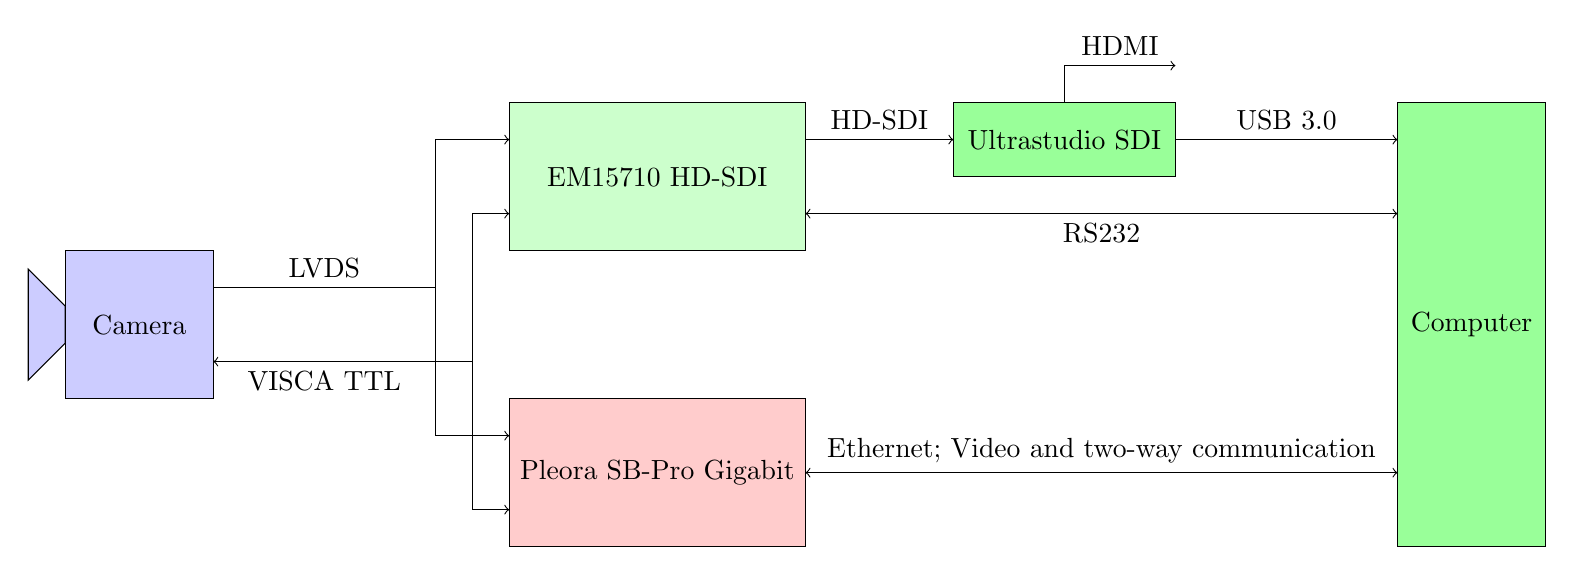
\begin{tikzpicture}[scale=0.94]
		% Camera
		\filldraw[fill=blue!20!white] (0,1) rectangle (2,-1);
		\filldraw[fill=blue!20!white] (0,0.25) -- (-0.5,0.75) -- (-0.5,-0.75) -- (0,-0.25) -- (0,0.25);
		\filldraw[fill=blue!20!white,draw=blue!20!white] (-0.1,-0.25) rectangle (0,.1,0.25);
		\node() at (1,0) {Camera};
		
		% EM
		\filldraw[fill=green!20!white] (6,1) rectangle (10,3);
		\node() at (8, 2) {EM15710 HD-SDI};
		
		% PL
		\filldraw[fill=red!20!white] (6,-1) rectangle (10,-3);
		\node() at (8, -2) {Pleora SB-Pro Gigabit};
		
		% U-SDI
		\filldraw[fill=green!40!white] (12,2) rectangle (15,3);
		\node() at (13.5, 2.5) {Ultrastudio SDI};
		
		% PC
		\filldraw[fill=green!40!white] (18,-3) rectangle (20,3);
		\node() at (19,0) {Computer};
		
		% Signal lines from camera
		\draw[] (2, 0.5) -- (5, 0.5) node [midway, above] {LVDS};
		\draw[->] (5, -0.5) -- (2, -0.5) node [midway, below] {VISCA TTL};
		
		% Signal lines to EM
		\draw[->] (5, 0.5) -- (5, 0.5) -- (5, 2.5) -- (6, 2.5);% LVDS
		\draw[->] (5, -0.5) -- (5.5, -0.5) -- (5.5, 1.5) -- (6, 1.5); % TTL
		
		% Signal lines to PL
		\draw[->] (5, 0.5) -- (5, 0.5) -- (5, -1.5) -- (6, -1.5); % LVDS
		\draw[->] (5, -0.5) -- (5.5, -0.5) -- (5.5, -2.5) -- (6, -2.5); % TTL
		
		% Signal line from EM to U-SDI
		\draw[->] (10,2.5) -- (12, 2.5) node [midway, above]{HD-SDI};
		
		% Signal line from U-SDI, HDMI
		\draw[->] (13.5,3) -- (13.5, 3.5) -- (15, 3.5) node [midway, above]{HDMI};
				
		% Signal line from EM to PC
		\draw[<->] (10,1.5) -- (18, 1.5) node [midway, below]{RS232}; 
		
		% Signal line from U-SDI to PC
		\draw[->] (15, 2.5) -- (18, 2.5) node [midway, above]{USB 3.0};
		
		% Signal line from PL to PC
		\draw[<->] (10,-2) -- (18, -2) node [midway, above]{Ethernet; Video and two-way communication}; 
	\end{tikzpicture}
	\caption{Schematics of the hardware}
	\label{fig:hw.schema}
\end{sidewaysfigure}